\begin{flushright} {\tiny {\color{gray} (tikz\_q22d.tex)}} \end{flushright}
%~~~~~~~~~~~~~~~~~~~~~~~~~~~~~~~~~~~~~~~~~~~~~~~~~~~~~~~~~~~~~~~~~~~~~~~~~~~~~~~~~~~~~~~~~~~~~~~~~~

\begin{center}
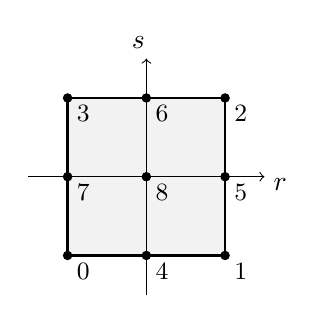
\begin{tikzpicture}
%\draw[step=0.5cm,gray,very thin] (0,0) grid (4,4); 
\draw[fill=gray!10,gray!10](1,1) rectangle (3,3);
\draw[thick] (1,1)--(3,1)--(3,3)--(1,3)--cycle;
\draw [->] (0.5,2) -- (3.5,2);
\draw [->] (2,0.5) -- (2,3.5);
\node[] at (3.7,1.9) {$r$};
\node[] at (1.9,3.7) {$s$};
\draw[black,fill=black] (1,1)   circle (1.5pt);
\draw[black,fill=black] (1,2)   circle (1.5pt);
\draw[black,fill=black] (1,3)   circle (1.5pt);
\draw[black,fill=black] (2,1)   circle (1.5pt);
\draw[black,fill=black] (2,2)   circle (1.5pt);
\draw[black,fill=black] (2,3)   circle (1.5pt);
\draw[black,fill=black] (3,1)   circle (1.5pt);
\draw[black,fill=black] (3,2)   circle (1.5pt);
\draw[black,fill=black] (3,3)   circle (1.5pt);
\node[] at (1.2,0.8) {\small $0$};
\node[] at (2.2,0.8) {\small $4$};
\node[] at (3.2,0.8) {\small $1$};
\node[] at (1.2,1.8) {\small $7$};
\node[] at (2.2,1.8) {\small $8$};
\node[] at (3.2,1.8) {\small $5$};
\node[] at (1.2,2.8) {\small $3$};
\node[] at (2.2,2.8) {\small $6$};
\node[] at (3.2,2.8) {\small $2$};
\end{tikzpicture}
\end{center}

